%%%%%%%%%%%%%%%%%%%%%%%%%%%%%%%%%%%%%%%%%%%%%%%%%%
%%%%% General setting %%%%%
%%%%%%%%%%%%%%%%%%%%%%%%%%%%%%%%%%%%%%%%%%%%%%%%%%
\documentclass[t]{beamer}
\usecolortheme{default}
\usetheme{default}

%% Vietnamese %%
% \usepackage[utf8]{vietnam}
%%%%%%%%%%%%%%%%%%%%%%%%%%%%%%%%%%%%%%%%%%%%%%%%%%



%%%%%%%%%%%%%%%%%%%%%%%%%%%%%%%%%%%%%%%%%%%%%%%%%%
%%%%% Tikz %%%%%
%%%%%%%%%%%%%%%%%%%%%%%%%%%%%%%%%%%%%%%%%%%%%%%%%%
\usepackage{pgfplots} %%%%%% Regression %%%%
\pgfplotsset{compat = newest}
\usepackage{pgfplotstable}
\usepackage{tikz}
\usepackage{tikz-3dplot} %%%%%% Draw %%%%%%
\usepackage{tikz,tkz-euclide}
\usetikzlibrary{arrows,calc,patterns}
% \usetikzlibrary{quotes,angles}
%\usetikzlibrary{shapes.geometric}
\usepackage{circuitikz} %%%%% Circuit %%%%
%\usetikzlibrary{decorations.pathmorphing,patterns}

%%%%%%%%%%%%%%%%%%%%%%%%%%%%%%%%%%%%%%%%%%%%%%%%%%

%% Color %%
\definecolor{BlueDefault}{rgb}{0.2,0.2,0.7}


%%%%%%%%%%%%%%%%%%%%%%%%%%%%%%%%%%%%%%%%%%%%%%%%%%
%%%%% Figure and Table %%%%%
%%%%%%%%%%%%%%%%%%%%%%%%%%%%%%%%%%%%%%%%%%%%%%%%%%

\usepackage{graphicx} % Required for inserting images

%% Caption of Figure and Table %%
\usepackage{caption}
% \captionsetup[figure]{labelsep=space,justification=centering}
% \captionsetup[table]{labelsep=space,justification=centering}

% Column, Row and Minipage %%
% \usepackage{minipage}

%%%%%%%%%%%%%%%%%%%%%%%%%%%%%%%%%%%%%%%%%%%%%%%%%%


%%%%%%%%%%%%%%%%%%%%%%%%%%%%%%%%%%%%%%%%%%%%%%%%%%
%%%%% General Information %%%%%
%%%%%%%%%%%%%%%%%%%%%%%%%%%%%%%%%%%%%%%%%%%%%%%%%%
\title{Antenna Fundamentals}
\author{Nguyen Thanh Long}
\institute{RF3i - Smart Sensor Lab}
% \date{\today}
\date{}
%%%%%%%%%%%%%%%%%%%%%%%%%%%%%%%%%%%%%%%%%%%%%%%%%%

%% Make Table of Contents %%
\AtBeginSection[]{
  \begin{frame}
  \frametitle{Outline}
  \tableofcontents[currentsection]
  \end{frame}
}

%% Section numbering %%
\setbeamertemplate{section in toc}[sections numbered]
\setbeamertemplate{subsection in toc}[subsections numbered]


%%%%%%%%%%%%%%%%%%%%%%%%%%%%%%%%%%%%%%%%%%%%%%%%%%
%%%%% Headline & Footline %%%%%
%%%%%%%%%%%%%%%%%%%%%%%%%%%%%%%%%%%%%%%%%%%%%%%%%%

%% Make page number %%
\setbeamertemplate{footline}[page number]

%% Headline %%
\setbeamertemplate{headline}
{
    \begin{beamercolorbox}{section in head/foot}
    % \vskip2pt\insertnavigation{\paperwidth}\vskip2pt
    \vskip2pt\insertsectionnavigationhorizontal{.5\textwidth}{\hskip0pt plus1filll}{}\vskip2pt
    
    \end{beamercolorbox}
}

%% Footline %%
\setbeamertemplate{footline}
{
    \hbox{%
  
    \begin{beamercolorbox}[wd=.333333\paperwidth,ht=2.25ex,dp=1ex,center]{author in head/foot}%
        \usebeamerfont{author in head/foot}\insertshortauthor
    \end{beamercolorbox}%
  
    \begin{beamercolorbox}[wd=.333333\paperwidth,ht=2.25ex,dp=1ex,center]{title in head/foot}%
        \usebeamerfont{title in head/foot}\insertshorttitle
    \end{beamercolorbox}%
  
    \begin{beamercolorbox}[wd=.333333\paperwidth,ht=2.25ex,dp=1ex,right]{date in head/foot}%
        \usebeamerfont{date in head/foot}\insertshortdate{}\hspace*{2em}
        \usebeamerfont{page number in head/foot}\insertframenumber{} / \inserttotalframenumber\hspace*{2ex}
    \end{beamercolorbox}}%
  
    \vskip0pt%
}
%%%%%%%%%%%%%%%%%%%%%%%%%%%%%%%%%%%%%%%%%%%%%%%%%%

%%%%%%%%%%%%%%%%%%%%%%%%%%%%%%%%%%%%%%%%%%%%%%%%%%
%%%%% Mathematics %%%%%
%%%%%%%%%%%%%%%%%%%%%%%%%%%%%%%%%%%%%%%%%%%%%%%%%%
\usepackage{esint} % various fancy integral symbols
\usepackage{bm} % bf vector
\usepackage{siunitx}
%%%%%%%%%%%%%%%%%%%%%%%%%%%%%%%%%%%%%%%%%%%%%%%%%%

%%%%%%%%%%%%%%%%%%%%%%%%%%%%%%%%%%%%%%%%%%%%%%%%%%
%%%%% Biblioraphy %%%%%
%%%%%%%%%%%%%%%%%%%%%%%%%%%%%%%%%%%%%%%%%%%%%%%%%%
\usepackage[backend=biber,style=ieee]{biblatex}
\addbibresource{Antenna_Fundamentals.bib}

\usepackage{url}
\usepackage{hyperref}
\hypersetup{
	colorlinks=true,
	linkcolor=black,
	filecolor=blue,
    citecolor=purple,
	urlcolor=blue,
	pdftitle={Overleaf Example},
	pdfpagemode=FullScreen,
}
%%%%%%%%%%%%%%%%%%%%%%%%%%%%%%%%%%%%%%%%%%%%%%%%%%


\begin{document}

% \maketitle
\frame{\titlepage}

\section{Time domain and Frequency domain}

\begin{frame}{Frequency domain}
    \begin{itemize}
        \item Fourier series: \( S(t) = \sum_{i=-\infty}^\infty s_i \exp \left( i \omega t \right). \)
        \item Time domain transform to frequency domain:
    \end{itemize}
    \vspace{3mm}
    \begin{tikzpicture}[scale=1]
        \draw 
        (-4,0) node{Time domain}
        (4,0) node{Frequency domain}
        (-4,-1) node{\( \dfrac{\partial }{\partial t} \)}
        (4,-1) node{\( j \omega \)}
        (-4,-2) node{\(x = x_0 \cos( \omega t + \varphi ) \)}
        (4,-2) node{\( x = x_0 \exp ( j \varphi ) \)}
        (4,-2.5) node{(Ignore \(\exp(j \omega t ) \) )}
        (0,0.4) node{Fourier transform}
        % (0,-0.6) node{Fourier transform}
        ;
        \draw[thick, -Stealth] (-2,0) to (2,0);
        \draw[thick, -Stealth] (-2,-1) to (2,-1);
        \draw[thick, -Stealth] (-2,-2) to (2,-2);
    \end{tikzpicture}
    \vspace{1mm}
    
    \textbf{Frequency is only continuous in the mindset of engineering, not mathematics and machinery. }
    
\end{frame}

\section{Ideal dipole problem}

\subsection{Solution of ideal dipole problem}

\begin{frame}{Solution of ideal dipole problem}
    \begin{columns}
        \column{0.4\textwidth}
        \vspace{-4mm}
        
        With \( \beta = \omega/c \), \( \eta = \sqrt{\mu/\varepsilon}\) \\
        
        \vspace{2mm}
        
        The vector Potential is
        \begin{align*}
            \mathbf{A} & = \iiint_{v'} \mu \mathbf{J} \dfrac{ \exp( - j \beta R ) }{ 4 \pi R } \mathrm{d} v' \\
            & = \dfrac{ \mu I \exp( - j \beta r ) }{ 4 \pi R} L \mathbf{\hat{z}}.
        \end{align*}

        \begin{itemize}
            \item Magnetic fields:
        \end{itemize}
        \begin{equation*}
            \mathbf{H} = \dfrac{1}{\mu} \nabla \times \mathbf{A}.
        \end{equation*}

        \begin{itemize}
            \item Electric fields:
        \end{itemize}
        \begin{equation*}
            \mathbf{E} = \dfrac{1}{j \omega \epsilon} \nabla \times \mathbf{H}.
        \end{equation*}
        
        \column{0.6\textwidth}
        \vspace{-4mm}
        \begin{equation*}
            I(z') = \left\{
            \begin{array}{ll}
                I_0 & x'=0, y'=0, \lvert z' \rvert \le L/2.  \\
                0 & \text{everywhere else}.
            \end{array}
            \right.
        \end{equation*}
        
        \begin{figure}
            \centering
            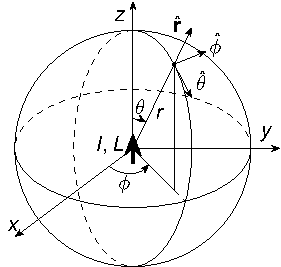
\includegraphics[width=0.7\textwidth]{Figures/Dipole_in_sphere_coordinate.pdf}
            \caption{Ideal dipole in sphere coordinate.}
            \label{fig:Ideal_dipole}
        \end{figure}
    \end{columns}
\end{frame}

%% Slide 2

\begin{frame}{Solution of ideal dipole problem}

    \vspace{-6mm}
    
    \begin{align*}
        \mathbf{A} = & \dfrac{\mu I \exp (-j \beta r)}{4 \pi r} L \mathbf{\hat{z}}, \\
        & \\
        \mathbf{H} = & \dfrac{I L}{4\pi} j \beta \left( 1 + \dfrac{1}{j \beta r} \right) \dfrac{ \exp ( - j \beta r) }{r} \sin \theta \mathbf{ \hat{\phi} }, \\
        & \\
        \mathbf{E} = & \dfrac{I L}{4\pi} j \omega \mu \left[ 1 + \dfrac{1}{j \beta r} - \dfrac{1}{(\beta r)^2} \right] \dfrac{ \exp ( - j \beta r) }{r} \sin \theta \mathbf{ \hat{\theta} } \\
        &+ \dfrac{I L}{2\pi} \eta \left[ \dfrac{1}{r} - j \dfrac{1}{\beta r^2} \right] \dfrac{ \exp ( - j \beta r) }{r} \cos \theta \mathbf{ \hat{r} }, \\
        & \\
        \mathbf{S} = & \dfrac{1}{2} \mathbf{E} \times \mathbf{H}^*.
    \end{align*}
\end{frame}

\subsection{Near field}

\begin{frame}{Near field}
    \begin{columns}
        \column{0.6\textwidth}
        Condition: \( \beta r \ll 1 \) or \( r \ll \lambda \). 
        \begin{itemize}
            \item Electromagnetic fields:
        \end{itemize}
        \begin{align*}
            \mathbf{H} &= \dfrac{ I L \exp ( -j \beta r ) }{4 \pi r^2} \sin \theta \mathbf{ \hat{\phi} }, \\
            \mathbf{E} &= - j \eta \dfrac{I L}{4 \pi \beta} \dfrac{\exp ( - j \beta r )}{r^3} \left( \sin \theta \mathbf{ \hat{\theta} } + 2 \cos \theta \mathbf{ \hat{r} } \right).
        \end{align*}
        \begin{itemize}
            \item Poynting vector:
        \end{itemize}
        \begin{equation*}
           \mathbf{S} = - \dfrac{ j \eta }{2 \beta} \left( \dfrac{I L}{4 \pi} \right)^2 \dfrac{1}{r^5} \left( \sin^2 \theta \mathbf{\hat{r}} - \sin 2 \theta \mathbf{\hat{\theta}} \right). 
        \end{equation*}
        
        \vspace{3mm}
        Power transfer by mutual induction.
        \column{0.4\textwidth}
        Near field properties:
        \begin{itemize}
            \item Electrostatic field.
            \item No Radiation Loss.
        \end{itemize}
        \begin{figure}
            \centering
            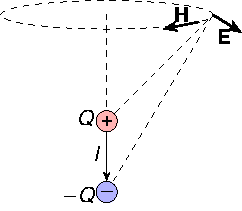
\includegraphics{Figures/Electrostatic_dipole.pdf}
            \caption{Electrostatic dipole model.}
            \label{fig:Electrostatic_diople}
        \end{figure}
    \end{columns}
\end{frame}



\subsection{Far field}
\begin{frame}{Far field}
    \begin{columns}
        \column{0.5\textwidth}
        Condition: \( r > L^2/2\lambda \) and \( r > 5 \lambda \)
        
        \begin{itemize}
            \item Electromagnetic fields:
        \end{itemize}
        \vspace{-2mm}
        \begin{align*}
            \mathbf{E} &= \dfrac{IL}{4 \pi} j \omega \mu \dfrac{ \exp ( - j \beta r) }{r} \sin \theta \mathbf{ \hat{\theta} }, \\
            \mathbf{H} &= \dfrac{IL}{4 \pi} j \beta \dfrac{ \exp ( - j \beta r) }{r} \sin \theta \mathbf{ \hat{\phi} }.
        \end{align*}

        \begin{itemize}
            \item Poynting vector:
        \end{itemize}
        \begin{equation*}
            \mathbf{S} = \dfrac{1}{2} \left( \dfrac{IL}{4 \pi} \right)^2 \omega \mu \beta \dfrac{\sin^2 \theta}{r^2} \mathbf{\hat{r}}.
        \end{equation*}
        
        \vspace{3mm}
        % In the far field, electromagnetic wave is the Spherical wave.
        \column{0.5\textwidth}
        \vspace{-6mm}
        \begin{itemize}
            \item Radiation loss power:
        \end{itemize}
        \begin{equation*}
            P_f = \iint \mathbf{S} \cdot \mathrm{d} \mathbf{s} = \dfrac{\omega \mu \beta}{12\pi} (I L)^2.
        \end{equation*}
        \vspace{-3mm}
        \begin{figure}
            \centering
            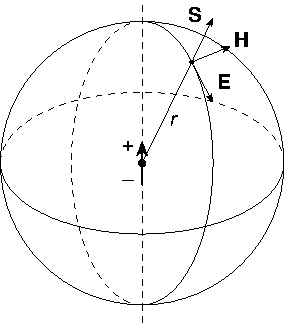
\includegraphics[width=0.75\textwidth]{Figures/Spherical_wave.pdf}
            \caption{Radiation in far fields.}
            \label{fig:Spherical_wave}
        \end{figure}
    \end{columns}
\end{frame}

\subsection{Radiation pattern}

\begin{frame}{Steps in the Evaluation of Radiation Fields}
\begin{columns}
    \column{0.6\textwidth}
    \cite{Stutzman_1998}
    \vspace{3mm}
    \begin{itemize}
        \item \textbf{Step 1: Find \(\mathbf{A}\).} 
        \begin{equation*}
            \mathbf{A} = \mu \dfrac{ \exp( - j \beta r ) }{ 4 \pi r } \iiint_{v'} \mathbf{J} \exp( - j \beta \mathbf{r} \cdot \mathbf{\hat{r}} )\mathrm{d} v'.
        \end{equation*}
        \item \textbf{Step 2: Find \(\mathbf{E}\).} 
        \begin{equation*}
            \mathbf{E} = -j\omega \mathbf{A} - ( -j\omega \mathbf{A} \cdot \mathbf{\hat{r}} ) \mathbf{\hat{r}}.
        \end{equation*}
        \item \textbf{Step 3: Find \(\mathbf{H}\).} 
        \begin{equation*}
            \mathbf{H} = \dfrac{1}{\eta} \hat{r} \times \mathbf{E}.
        \end{equation*}
    \end{itemize}
    \column{0.4\textwidth}
    \begin{figure}
        \centering
        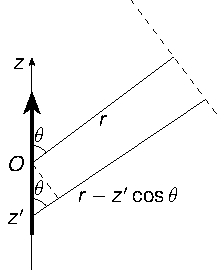
\includegraphics[width=0.9\textwidth]{Figures/Interference.pdf}
        \caption{Interference of electromagnetic waves}
        \label{fig:Interference}
    \end{figure}
\end{columns}
\end{frame}

\begin{frame}{Radiation pattern}
    \begin{columns}
        \column{0.5\textwidth}
            Fields of uniform line source
        \begin{align*}
            A_z &= \dfrac{ \exp ( -j \beta r) }{4 \pi r} \int_{-L/2}^{L/2} I(z') \exp( j \beta z') \mathrm{d}z' \\
            &= \dfrac{ \exp ( -j \beta r) }{4 \pi r} \dfrac{\sin [(\beta L/2) \cos (\theta)]}{(\beta L/2) \cos (\theta)}. \\
            \mathbf{E} &= j \omega \sin \theta A_z \mathbf{\hat{\theta}}.
        \end{align*}
        
        Radiation pattern:
        \begin{align*}
            &F(\theta,\phi) = \dfrac{E(\theta,\phi)}{E_{max}} = g(\theta) f(\theta,\phi) \\
            &= \sin \theta \cdot \dfrac{\sin [(\beta L/2) \cos (\theta)]}{(\beta L/2) \cos (\theta)}.
        \end{align*}
        \column{0.5\textwidth}
        \begin{figure}
            \centering
            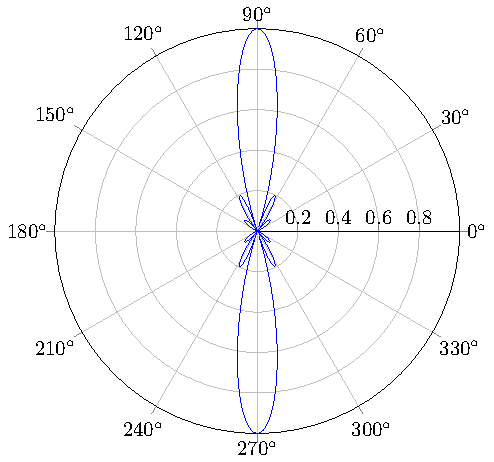
\includegraphics[width=\textwidth]{Figures/Radiation_pattern_diagram/Polar_plot.pdf}
            \caption{Radiation pattern with \( \beta L/2 = 10\).}
            \label{fig:Polar_radiation_pattern}
        \end{figure}
    \end{columns}
\end{frame}

\section{Antenna Performance Parameters}

\subsection{Directivity and Gain}
\begin{frame}{Directivity and Gain}
    \cite{Balanis_2012} \cite{Kraus-2002-AntennasB}
    \begin{columns}
        \column{0.5\textwidth}
            \begin{itemize}
                \item Radiation density
            \end{itemize}
            \begin{equation*}
                U = \dfrac{\text{Power}}{\text{Solid angle}} = S r^2,
            \end{equation*}
            % or
            \begin{equation*}
                U (\theta, \phi) = U_m \left| F(\theta, \phi) \right|^2.
            \end{equation*}

            \begin{itemize}
                \item Directivity
            \end{itemize}
            \begin{equation*}
                D = \dfrac{U_m}{U_{ave}}.
            \end{equation*}
            
            \begin{itemize}
                \item Gain
            \end{itemize}
            \begin{equation*}
                G = e_r D,
            \end{equation*}
            where \(e_r\) is efficiency.
        \column{0.5\textwidth}
        \begin{figure}
            \centering
            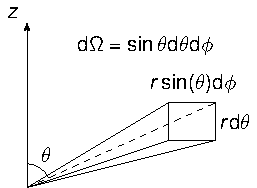
\includegraphics[width=\textwidth]{Figures/Solid_angle.pdf}
            \caption{Solid andgle.}
            \label{fig:Solid_angle}
        \end{figure}
    \end{columns}
\end{frame}

\subsection{Impedance and Efficiency}

\begin{frame}{Impedance and Efficiency}
    \vspace{-6mm}
    \begin{columns}
        \column{0.4\textwidth}
        \begin{itemize}
            \item Impedance
        \end{itemize}
        \begin{equation*}
            R_r = \dfrac{2P}{I^2} = \dfrac{2\pi}{3} \eta \left( \dfrac{L}{\lambda} \right)^2.
        \end{equation*}
        \vspace{-3mm}
        \begin{itemize}
            \item Efficiency
        \end{itemize}
        \begin{equation*}
            e_r = \dfrac{P_r}{P_{in}} = \dfrac{R_r}{R_r+R_o}.
        \end{equation*}
        \vspace{-6mm}
        \begin{figure}
            \centering
            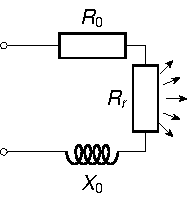
\includegraphics[width=0.6\textwidth]{Figures/Antenna_circuit.pdf}
            \caption{Antenna equivalent circuit.}
            \label{fig:Antenna_circuit}
        \end{figure}
        
        \column{0.6\textwidth}
        \begin{itemize}
            \item  Ohmic resistance for an antenna
        \end{itemize}
        \vspace{-3mm}
        \begin{figure}
            \centering
            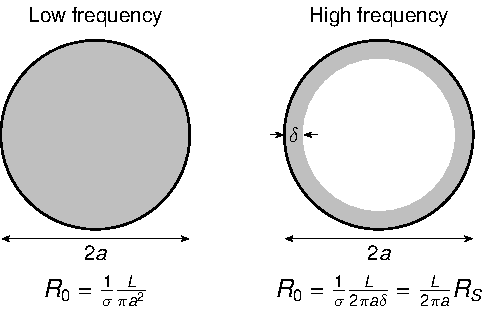
\includegraphics[width=\textwidth]{Figures/Skin_effect.pdf}
            \caption{Skin effect in high frequency.}
            \label{fig:Skin_effect}
        \end{figure}
        where \(\delta = \sqrt{2/ \omega \mu \sigma}\), \( R_S = \sqrt{\omega \mu / 2 \sigma }\).        
    \end{columns}
\end{frame}

\section{Simple Radiating Systems}

\documentclass{standalone}

\usepackage[OT1]{fontenc}
\renewcommand*\familydefault{\sfdefault}
\usepackage{helvet,sfmath}
\usepackage{siunitx}

\usepackage{tikz}
\usetikzlibrary{arrows,calc,patterns}
\usepackage{tikz,tkz-euclide}

\definecolor{BlueDefault}{rgb}{0.2,0.2,0.7}

\begin{document}

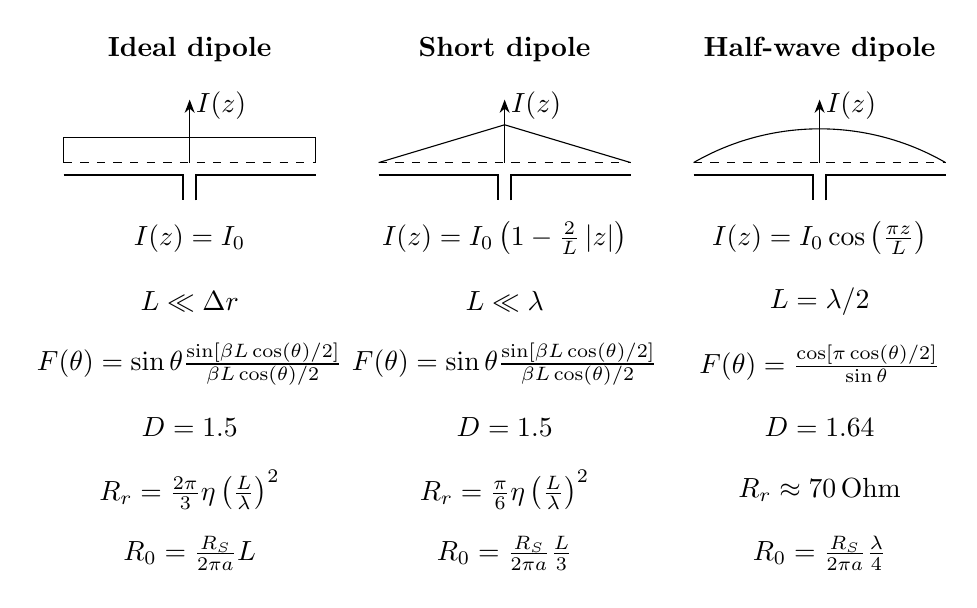
\begin{tikzpicture}[scale=0.8]
    %% Dipoles
    \foreach \x in {-5,0,5}
    {
    \draw[thick]
    (\x-2,0) to (\x-0.1,0) to (\x-0.1,-0.4)
    (\x+0.1,-0.4) to (\x+0.1,0) to (\x+2,0)
    ;
    
    \draw[-Stealth]
    (\x,0.2) to (\x,1.2)
    ;

    \draw[dashed]
    (\x-2,0.2) to (\x+2,0.2)
    ;
    
    \draw
    (\x+0.5,1.1) node{\(I(z)\)}
    ;
    }
    %% Ideal dipole
    \draw
    (-3,0.2) to (-3,0.6) to (-7,0.6) to (-7,0.2)
    ;
    \draw
    (-5,2) node{\textbf{Ideal dipole}}
    ;
    \draw
    (-5,-1) node{\(I(z) = I_0\)}
    (-5,-2) node{\(L \ll \Delta r\)}
    (-5,-3) node{\( F(\theta) = \sin \theta \frac{ \sin \left[ \beta L \cos ( \theta )/2 \right]}{ \beta L \cos ( \theta )/2} \)}
    (-5,-4) node{\(D=1.5\)}
    (-5,-5) node{\(R_r = \frac{2\pi}{3} \eta \left( \frac{L}{\lambda} \right)^2\)}
    (-5,-6) node{\(R_0 = \frac{R_S}{2\pi a} L\)}
    ;
    %% Short dipole
    \draw
    (2,0.2) to (0,0.8) to (-2,0.2)
    ;
    \draw
    (0,2) node{\textbf{Short dipole}}
    ;
    \draw
    (0,-1) node{\( I(z) = I_0 \left( 1 - \frac{2}{L} \left| z \right| \right) \)}
    (0,-2) node{\(L \ll \lambda\)}
    (0,-3) node{\( F(\theta) = \sin \theta \frac{ \sin \left[ \beta L \cos ( \theta )/2 \right]}{ \beta L \cos ( \theta )/2} \)}
    (0,-4) node{\(D=1.5\)}
    (0,-5) node{\(R_r = \frac{\pi}{6} \eta \left( \frac{L}{\lambda} \right)^2\)}
    (0,-6) node{\(R_0 = \frac{R_S}{2\pi a} \frac{L}{3}\)}
    ;
    %% Half-wavelenght antenna
    \draw
    (7,0.2) arc(60:120:4)
    ;
    \draw
    (5,2) node{\textbf{Half-wave dipole}}
    ;
    \draw
    (5,-1) node{\( I(z) = I_0 \cos \left( \frac{\pi z}{L} \right) \)}
    (5,-2) node{\(L = \lambda/2\)}
    (5,-3) node{\( F(\theta) = \frac{ \cos \left[ \pi \cos (\theta) /2 \right] }{\sin \theta} \)}
    (5,-4) node{\(D=1.64\)}
    (5,-5) node{\(R_r \approx \SI{70}{Ohm}\)}
    (5,-6) node{\(R_0 = \frac{R_S}{2\pi a} \frac{\lambda}{4}\)}
    ;
\end{tikzpicture}

\end{document}

\documentclass{standalone}

\usepackage[OT1]{fontenc}
\renewcommand*\familydefault{\sfdefault}
\usepackage{helvet,sfmath}
\usepackage{siunitx}

\usepackage{tikz}
\usetikzlibrary{arrows,calc,patterns}
\usepackage{tikz,tkz-euclide}


\definecolor{BlueDefault}{rgb}{0.2,0.2,0.7}

\begin{document}

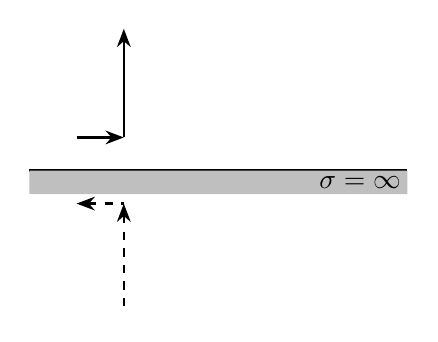
\begin{tikzpicture}[scale=0.6]
    %% Ground
    \draw[very thick] (0,0) to (8,0);
    \draw[draw=none, fill=lightgray] (0,0) to (8,0) to (8,-0.5) to (0,-0.5) to (0,0);
    \draw (7.0,-0.25) node{\(\sigma = \infty \)};
    %% Antenna
    \draw[thick, -Stealth] (1,0.7) to (2,0.7);
    \draw[thick, -Stealth] (2,0.7) to (2,3);
    \draw[dashed, thick, Stealth-] (1,-0.7) to (2,-0.7);
    \draw[dashed, thick, Stealth-] (2,-0.7) to (2,-3);
    
\end{tikzpicture}    

\end{document}

\subsection{Small loop antenna}

\begin{frame}{Small loop antenna}
    \begin{columns}
        \column{0.5\textwidth}
        \begin{align*}
            \mathbf{A} &= \dfrac{\mu l_1 I}{4 \pi} \left[ \dfrac{\exp ( - j \beta r_1 )}{r_1} - \dfrac{\exp ( - j \beta r_3 )}{r_3} \right] \mathbf{\hat{x}} \\
            &+ \dfrac{\mu l_2 I}{4 \pi} \left[ \dfrac{\exp ( - j \beta r_2 )}{r_2} - \dfrac{\exp ( - j \beta r_4 )}{r_4} \right] \mathbf{\hat{y}} \\
            & \approx j \beta S \dfrac{\mu I}{4\pi} \dfrac{\exp ( - j \beta r )}{r} \sin \theta \mathbf{\hat{\phi}}.
        \end{align*}
        
        \vspace{3mm}
        Note: \( r_1-r_3 = \Delta r_{13} \approx l_2 \cos \theta \ll r_i \)
        \begin{align*}
            \Rightarrow f(r_1) - f(r_3) &= f'(r) \cdot \Delta r_{13}. \\
            &= \nabla f(r) \cdot \Delta \mathbf{r}_{13}.
        \end{align*}
        \column{0.5\textwidth}
        \vspace{-8mm}
        \begin{figure}
            \centering
            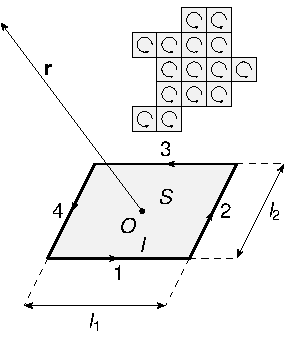
\includegraphics[width=\textwidth]{Figures/Small_loop.pdf}
            \caption{Rectangle small loop antenna.}
            \label{fig:small_loop}
        \end{figure}
    \end{columns}
\end{frame}

\begin{frame}[allowframebreaks]{bibliography}

\printbibliography

\end{frame}



\end{document}
